\chpt{Introduction} \label{chpt:intro}

\section{Human microbiome}
We are living in an environment that is full of microorganisms such as bacteria, fungus and virus. It is hard for humans to notice the existences of those small living creatures but they are everywhere.  The human body is one of major habitats for those microorganisms. It is well known that hundreds of thousands of microbes are residing on or in the human body such as skin, mouth, gut and vagina. The total number of bacterial cells over the human body is estimated to be $10^{14}$, which is ten times more than the number of human cells. The term, "microbiome", is used to refer to the totality of microbes and their genomes. Different human body sites show distinctive microbiome composition. For example, the human gut is dominated by Firmicutes and Bacteroidetes, while the skin is primarily inhibited by Actinobacteria and Bacteroidetes \citep{Cho:2012cn}. Substantial interpersonal and temporal variation of microbiome composition are also observed in many microbiome studies \citep{turnbaugh2007human}. The variation of the microbiome composition is possibly due to host genetics \citep{Knights:2014jta}, physiology \citep{Sommer:2013hq}, lifestyle \citep{wu2011linking} and environment \citep{Adams:2015ga}. Since the considerable amount of microbes over the human body are crucial to human health, they are often considered as another human organ.

The microbiome plays a critical role in human health. Some of the microbes are beneficial to human health. For instance, probiotic bifidobacteria can protect the host from lethal infection \citep{Fukuda:2012hg}. Faecalibacterium prausnitzii is found to have anti-inflammatory effect and can guard the host from intestinal inflammation \citep{Sokol:2008ke}. Bacteroides and other intestinal bacteria are essential for carbohydrate fermentation in the human gut. The product, fatty acids, generated from those microbes are then absorbed by human gut as an energy source \citep{Wexler:2007cn}. However, not all microbes are promoting good health for humans. Some of them are detrimental. For example, infection of Clostridium difficile can cause inflammation, bleeding and diarrhea, which is life-threatening and kills thousands of people in the United States each year \citep{Lessa:2015wl}. E.coli O157:H7, which is a specific strain of Escherichia coli, can cause diarrhea, abdominal pain, fever, dehydration, and sometimes kidney failure. It is estimated that this pathogen causes about 2,100 hospitalizations and 60 deaths in the United States each year \citep{Berkenpas:2006wl}. In 2011, the outbreak of  E.coli O104:H4, another strain of Escherichia coli,  caused hundreds of people to be admitted to hospital and resulted in several deaths in Germany. In order to decipher the function and impact of the microbes on the human well-being, great efforts have been made to develop new technology to study the microbiome in a more accurate and efficient way.

\section{High throughput sequencing approaches for microbiome studies}
Before the advent of high-throughput sequencing technologies, researchers studied the human microbiome by culturing the individual microbe. This approach has some disadvantages. First, most microbes have not been cultured. Therefore, those non-culturable microbes in the sample are difficult to study. Second, the traditional approach can only study a few microbes at a time and thus is not efficient to profile the whole microbial community. Next generation sequencing (NGS) technology has been widely used to explore the microbial community in order to understand their roles in human health and diseases. This sequencing approach can be applied to samples directly from patients without culturing the microbes. Thus this approach is especially useful for studying non-culturable microbes. Since the NGS technology can sequence millions of DNA sequences in a parallel fashion, it has the advantage to investigate a large number of microbes in a sample at the same time.


Currently, two NGS based approaches have been used in microbiome studies. Both approaches are powerful and have been widely used in human microbiome studies, such as the Human Microbiome Project (HMP) \citep{turnbaugh2007human} and the Metagenomics of the Human Intestinal Tract (MetaHIT) project \citep{qin2010human}. 

One approach is based on 16S ribosomal RNA (rRNA) sequencing, which sequences the 16S rRNA gene to profile the bacterial community. The 16S rRNA gene uniquely exists in prokaryotes and its high variability in microbial genomes can be exploited to identify different microbes. In this approach, researchers can design PCR primers based on the conserved region of the 16s rRNA gene to amplify part of the genomic region of this gene. The amplicons are then sequenced by high-throughput sequencing technology. The sequencing reads generated from the variable regions of the 16s rRNA gene can be use for taxonomic classification and abundance quantification. However, the 16S data are limited in discerning the bacteria at the species or strain level. Also, the PCR amplification would introduce bias and thus affect the accuracy of abundance quantification. Since the 16S rRNA approach is cost effective and the data are relatively easy to analyze, it has been the most popular approach in microbiome studies. 

One important issue in 16S rRNA sequencing data analysis is how to identify the taxonomic origins of the 16S sequences. One strategy  is to align the obtained 16S sequences against the 16S databases such as Greengenes \citep{DeSantis:2006ii}, RDP \citep{Cole:2014jw} and SILVA \citep{Quast:2013hk}. Another strategy is to cluster the sequences into Operational Taxonomic Units (OTUs) with certain threshold. Each cluster is assumed to represent one taxon. For instances, with 97\% sequence similarity as the clustering threshold, the OTUs are considered to represent species.  After obtaining the OTUs and their taxonomic assignment, it is then followed by almost standard analysis such as distance based analysis, ordination (multiple dimensional scaling or principle component analysis), clustering and association analysis such as regression analysis. For an example of 16S rRNA data analysis, readers can refer to \citet{wu2011linking}. Several computational tools have been developed for 16S rRNA sequencing data analysis such as QIIME \citep{Caporaso:2010jf} and mothur \citep{Schloss:2009do}. The commonly used computational methods have been included in those softwares.



\begin{figure}[p]
	\begin{center}
		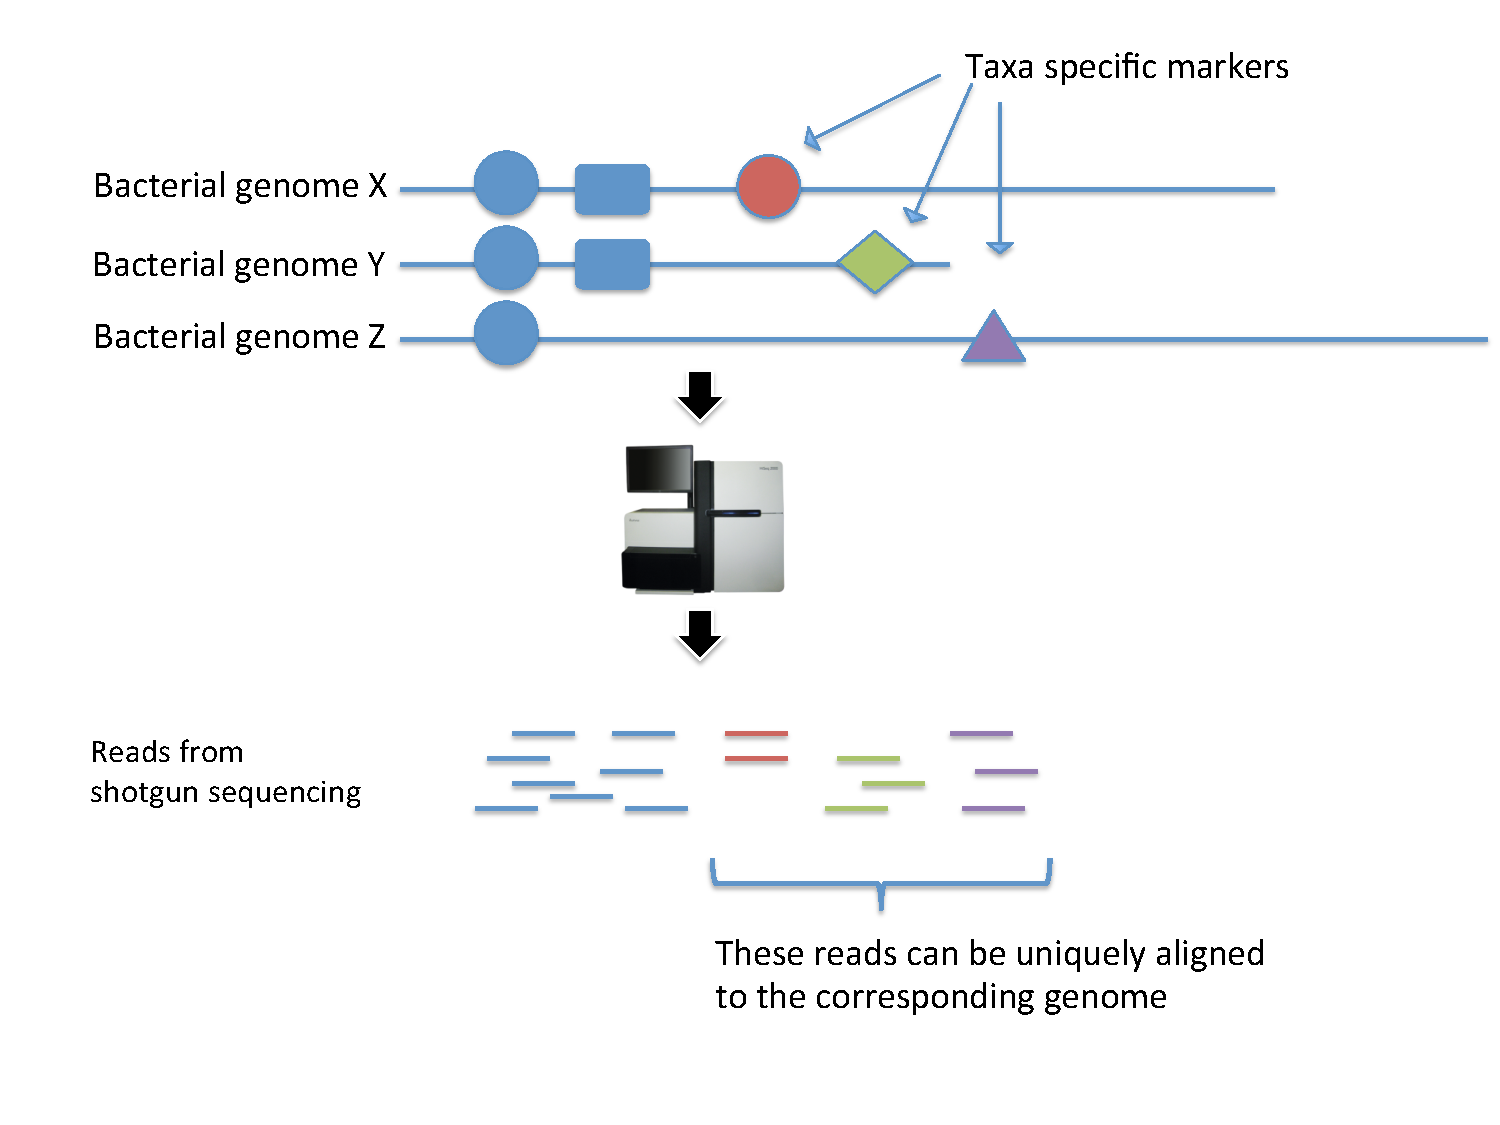
\includegraphics[scale=0.55,trim=0 0 0 0,clip]{Figure/F11_MetaPhlAn.pdf}
		\caption[An illustration of marker-based analysis strategy  for shotgun metagenomic data]{An illustration of marker-based analysis strategy  for shotgun metagenomic data. Taxa specific markers are identified by comparing known microbial genomes from public databases. Those taxa specific markers are then used as the reference for alignment. Reads that fail to be aligned to the markers are discarded. Reads that can be aligned are used for quantifying microbial abundance.} \label{F11_MetaPhlAn}
	\end{center}
\end{figure}


Alternatively, shotgun sequencing of metagenomes, which sequences all genome sequences presented in the sample instead of just one marker gene, provides a more comprehensive approach to study human microbiome. This approach provides richer information about the microbial composition and gene functions. However, the analysis for shotgun sequencing data is more challenging than 16S rRNA sequencing data. One great difficulty is how to quantify the microbial abundance. Since the sequencing reads are generated from whole genomes and microbial genomes share great similarity, it is difficult to uniquely align the reads back to the corresponding reference genomes. This makes the task of abundance quantification quite challenging. Currently, the most widely used strategy is to utilize  marker genes, either universal  markers \citep{Sunagawa:2013if} or taxa specific markers \citep{segata2012metagenomic}. For example, MetaPhlAn compared currently known microbial genomes from public databases and identified taxa specific markers \citep{segata2012metagenomic}. Those taxa specific markers are then used as the reference for alignment. Reads that fail to be aligned to the markers are discarded. Reads that can be aligned are used for quantifying microbial abundance. The marker-based analysis strategy used by MetaPhlAn is demonstrated in Figure~\ref{F11_MetaPhlAn}. In most current literatures, MetaPhlAn are used for shotgun metagenomic data analysis.



This dissertation is specifically focused on the analysis of shotgun metagenomic data as well as development of statistical models for shotgun metagenomic data. 


\section{Penn microbiome study of pediatric Crohn's disease}
Inflammatory bowel disease (IBD) is a disease involving chronic inflammation of gastrointestinal track. IBD can be categorized by the location of the inflammation to two forms, Crohn's disease (CD) and ulcerative colitis (UC). The symptoms of IBD include severe diarrhea, pain, fatigue and weight loss. The cause of the IBD is not entirely known although it is known to associate with abnormal host immune response. Recent studies show that the gut microbiome may play a role in the IBD onset \citep{gevers2014treatment} but the mechanism is not completely understood. Although treatments for IBD are available, currently there is no effective treatment to cure IBD without remission or relapse. One commonly used treatment is anti tumor necrosis factor (anti-TNF) treatment, which uses antibodies directed against host immune protein tumor necrosis factor $\alpha$ (TNF$\alpha$) to suppress immune response of the host. Anti-TNF treatment is not expected to alter the gut microbiome composition directly. It is reported to have side effects including increased risk of infection \citep{Borrelli:2006tk, Rutgeerts:2012ul}. Another treatment is enteral nutrition treatment, also called diet treatment, which feeds patients with defined formula diet. It possibly alters the gut microbiome composition. Diet treatment avoids immunosuppression but is difficult to maintain a long term effect \citep{Grover:2013dj}. The mechanisms of these treatments are not entirely clear.

\begin{figure}[p]
	\begin{center}
		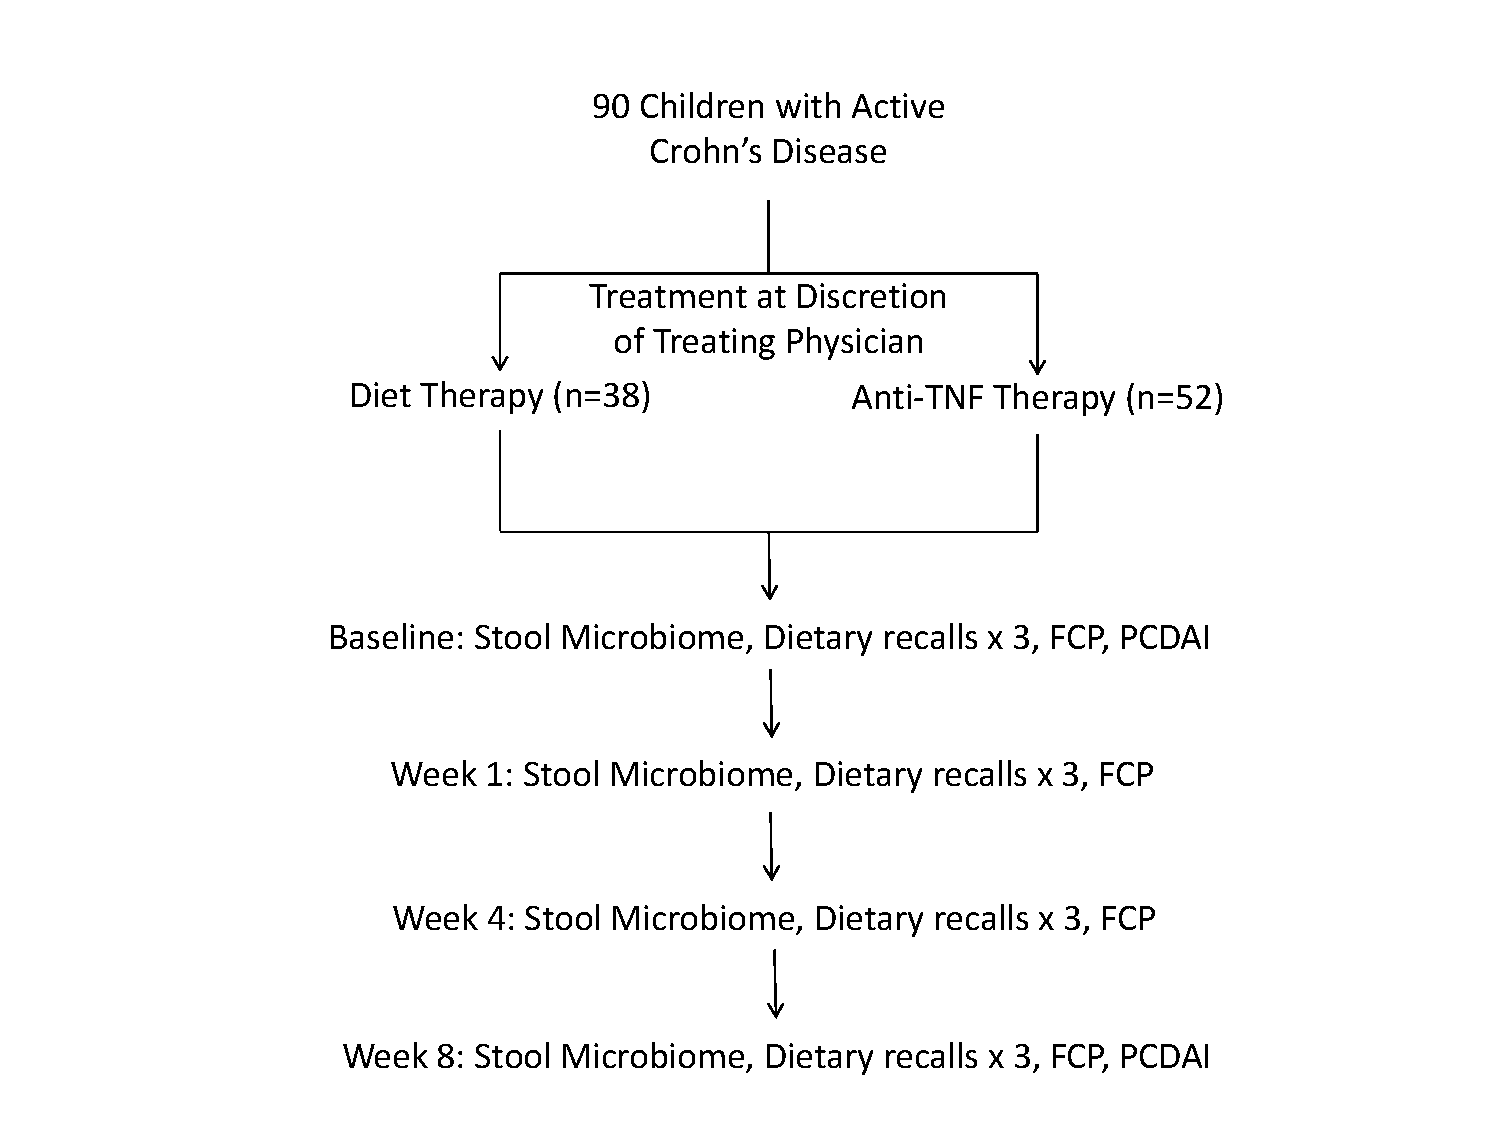
\includegraphics[scale=0.60,trim=40 0 0 0,clip]{Figure/F12_PLEASE_Study.pdf}
		\caption[An illustration of the PLEASE study at University of Pennsylvania.]{An illustration of the Penn PLEASE study. This is a collaborative work with Gary Wu (Department of Gastroenterology), Rick Bushman (Department of Microbiology), Jim Lewis (Department of Epidemiology) and people in their teams. PLEASE, Pediatric Longitudinal Study of Enteral Nutrition Therapy and Stool Microbiome Composition.} \label{F12_PLEASE_Study}
	\end{center}
\end{figure}




To improve our understanding of the role of human gut microbiome in Crohn's disease pathogenesis and how microbiome is associated with treatment response, we carried out a microbiome study called PLEASE  (Pediatric Longitudinal Study of Enteral Nutrition Therapy and Stool Microbiome Composition) at University of Pennsylvania (Penn) and The Children's Hospital of Philadelphia (CHOP). This is a collaborative work with Gary Wu (Department of Gastroenterology), Rick Bushman (Department of Microbiology), Jim Lewis (Department of Epidemiology) and people in their teams. The basic study design is demonstrated in Figure~\ref{F12_PLEASE_Study}.  In this study, we recruited a prospective cohort of pediatric Crohn's disease patients (ninety children) and collected their fecal samples as well as clinical data. The patients started therapy with either enteral nutrition or anti-TNF$\alpha$ antibodies (52 anti-TNF; 22 exclusive enteral nutrition [EEN]; 16 partial enteral nutrition with ad lib diet [PEN]). Stool samples were collected at four time points: baseline, 1 week, 4 weeks, and 8 weeks into therapy. We analyzed fecal samples using shotgun metagenomic sequencing approach.


\section{Dissertation organization }

The rest of the dissertation is structured as following. Chapter 2 presents the Penn microbiome study of pediatric Crohn's disease. In this project, we collected stool samples and clinical data from a prospective cohort of pediatric Crohn's disease patients, who started therapy with enteral nutrition or anti-TNF$\alpha$ antibodies. The fecal samples were analyzed by shotgun metagenomic sequencing approach. The results reveal the full complement and dynamics of bacteria and fungi during treatment. Bacterial community membership was associated independently with dysbiosis, intestinal inflammation, antibiotic use, and therapy.

Motived by the problems in the real data analysis, this dissertation also presents two statistical models for microbiome data analysis. Chapter 3 presents a multi-sample Poisson model to quantify microbial abundances. One important aspect of metagenomic data analysis is to quantify the bacterial abundances based on the sequencing data. In order to account for certain systematic differences in read coverage along the genome, we propose a multi-sample Poisson model to quantify microbial abundances based on read counts that are assigned to species-specific taxonomic markers. Our model takes into account the marker-specific effects when normalizing the sequencing count data in order to obtain more accurate quantification of the species abundances. 

Chapter 4 presents another statistical model  for longitudinal microbiome data analysis. A key question in longitudinal microbiome studies is to identify the microbes that are associated with clinical outcomes or environmental factors. We develop a zero-inflated Beta regression model with random effects (ZIBR) for testing the association between microbial abundance and clinical covariates for longitudinal microbiome data. The model includes a logistic regression component to model presence/absence of a microbe in samples and a Beta regression component to model non-zero microbial abundance, where each component includes a random effect to take into account the correlations among repeated measurements on the same subject. The statistical methods were evaluated using simulations as well as the real data from Penn microbiome study of pediatric Crohn's disease.

All the analysis included in this dissertation were carried out in a  reproducible research fashion. Chapter 5 briefly demonstrates the examples of reproducible research for the three projects presented in the dissertation.

Finally, we present conclusions and outline the future research directions in Chapter 6. The three projects presented in Chapters 2, 3 and 4 are self-contained. Readers who are interested in individual project can read the corresponding chapter without referring to other ones.
